\section{Deep Learning on Graphs}
\label{s_Background}

The foundation of this research lies at the intersection of graph theory, machine learning, and temporal data analysis. 
%This chapter provides a comprehensive overview of the key concepts and methodologies that underpin the thesis, and introduces the notation used throughout the thesis. 
This chapter acts as a guide, leading the reader through the key concepts and methodologies that underpin this thesis while introducing the notation used throughout.
A core preliminary for explaining deep graph models on dynamic graphs lies in dynamic graphs themselves. Thus, chapter \ref{s_Background_Graphs} establishes the definitions and foundational differences between static and dynamic graphs (Section \ref{s_Background_Graphs}). After that, geometric deep learning is outlined (Section \ref{s_Background_GeometricDeepLearning}) as the basis for deep graph models, followed by an in-depth introduction to \glspl{gnn} (Section \ref{s_Background_GNNs}). Building upon this foundation, the final sub-chapter (Section \ref{s_Background_TGNNs}) covers the extension of \glspl{gnn} into the temporal domain. It introduces \gls{gnn} models designed for different representations of dynamic graphs, which are the dominant deep model for dynamic graphs. 

\subsection{Graphs}
\label{s_Background_Graphs}
On the most fundamental level, graphs are a mathematical structure for modeling pairwise relationships between objects \cite{diestel_graph_2017}. They find application in diverse domains like social and communication networks \cite{bronstein_geometric_2017}. Graphs can be defined and notated in various ways. This thesis employs a notation influenced by Diestel \cite{diestel_graph_2017}, You et al. \cite{you_roland_2022}, and Souza et al. \cite{souza_provably_2022} to introduce and explore essential graph-related concepts.
% Introduction into the very basic definitions of graphs

A graph is characterized as a pair $G = (V, E)$, consisting of a set of vertices $V= \{v_1,...,v_n\}$, also called nodes, and a multi-set of edges $E \subseteq V \times V$ \cite{diestel_graph_2017, you_roland_2022}. Each edge $e \in E$ is associated with two vertices, which are called its ends \cite{diestel_graph_2017}. If a vertex $v \in V$ is and end of edge $e \in E$ then $v$ is designated as incident to $e$ \cite{diestel_graph_2017}. An edge $e \in E$ connecting a node $v \in V$ with itself is called a loop \cite{diestel_graph_2017}. Another vertex $u \in V$ is adjacent, or a neighbor, to vertex $v$ if they are connected by an edge \cite{diestel_graph_2017}. 

Two vertices $v_0, v_n \in V$ can be linked by a walk $W(v_0, v_n)$, which is an alternating sequence of vertices and edges $W(v_0, v_n)=(v_0, e_0, v_1, ..., e_n, v_n)$ so that for all $j=1,..,n$ the nodes $v_{j-1}$ and $v_j$ are the end points of edge $e_j$. The length of a walk is the number of edges in the walk \cite{diestel_graph_2017}.
% In the context of this work, we are interested in graphs that exhibit specific characteristics
These foundational definitions are extended to different graph types that play pivotal roles in different applications. These variants provide a richer vocabulary for modeling complex relationships and structures.

\begin{itemize}
    \item In a \textbf{directed graph} each edge $e \in E$ connecting vertices $u \in V$ and $v \in V$ has a designated stating point and end point \cite{diestel_graph_2017}. Therefore, it is represented as tuple $e = (u, v)$ with initial vertex $u$ and terminal vertex $v$. 
    \item In an \textbf{undirected graph}, edges have no direction, meaning that edge $e \in E$ connecting vertices $u \in V$ and $v \in V$ can be represented as set $e = \{u, v\}$.
    \item A \textbf{multigraph} is a type of graph where multi-edges are permitted. This means that for an edge $e_i = (u,v) \in E$ there could exist multiple other edges $e_j = (u,v) \in E$ that share the same ends \cite{kazemi_representation_2019}.
    \item An \textbf{attributed} graph associates properties with vertices and/or edges to represent their characteristics \cite{kazemi_representation_2019}. Node features are denoted as $F^{vertex} = \{f^{vertex}_v | v \in V\}$, and edge features as $F^{edge} = \{f^{edge}_e | e \in E\}$. 
    \item A graph is called \textbf{$r$-partite} if $V$ can be partitioned into $r$ classes so that all edges have their ends in different classes \cite{diestel_graph_2017}. A $2$-partite graph is generally referred to as \textbf{bipartite} \cite{diestel_graph_2017}.
\end{itemize}

\begin{figure}[h]
    \centering
\begin{subfigure}[b]{0.45\textwidth}
    \centering
    % TikZ code for the first graph
    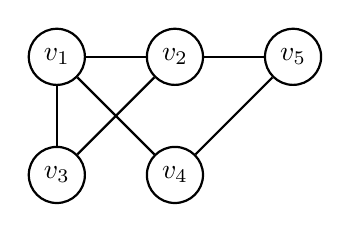
\begin{tikzpicture}[node distance={15mm}, thick, main/.style = {draw, circle}]
        \node[main] (1) {$v_1$};
        \node[main] (2) [right of=1] {$v_2$};
        \node[main] (3) [below of=1] {$v_3$};
        \node[main] (4) [below of=2] {$v_4$};
        \node[main] (5) [right of=2] {$v_5$};
        \draw (1) -- (2);
        \draw (1) -- (3);
        \draw (1) -- (4);
        \draw (2) -- (3);
        \draw (2) -- (5);
        \draw (4) -- (5);
    \end{tikzpicture}
    \caption{Undirected graph}
    \label{f_graphs_undirected}
\end{subfigure}
\begin{subfigure}[b]{0.45\textwidth}
    \centering
    % TikZ code for the second graph
    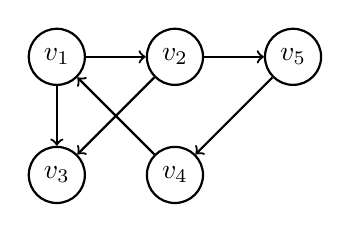
\begin{tikzpicture}[node distance={15mm}, thick, main/.style = {draw, circle}]
        \node[main] (1) {$v_1$};
        \node[main] (2) [right of=1] {$v_2$};
        \node[main] (3) [below of=1] {$v_3$};
        \node[main] (4) [below of=2] {$v_4$};
        \node[main] (5) [right of=2] {$v_5$};
        \draw[->] (1) -- (2);
        \draw[->] (1) -- (3);
        \draw[->] (4) -- (1);
        \draw[->] (2) -- (3);
        \draw[->] (2) -- (5);
        \draw[->] (5) -- (4);
    \end{tikzpicture}
    \caption{Directed graph}
    \label{f_graphs_directed}
\end{subfigure}
\par\bigskip
\begin{subfigure}[b]{0.45\textwidth}
    \centering
    % TikZ code for the first graph
    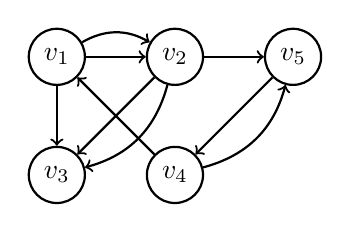
\begin{tikzpicture}[node distance={15mm}, thick, main/.style = {draw, circle}]
        \node[main] (1) {$v_1$};
        \node[main] (2) [right of=1] {$v_2$};
        \node[main] (3) [below of=1] {$v_3$};
        \node[main] (4) [below of=2] {$v_4$};
        \node[main] (5) [right of=2] {$v_5$};
        \draw[->] (1) -- (2);
        \draw[->] (1) to[bend left] (2);
        \draw[->] (1) -- (3);
        \draw[->] (4) -- (1);
        \draw[->] (2) -- (3);
        \draw[->] (2) to[bend left] (3);
        \draw[->] (2) -- (5);
        \draw[->] (5) -- (4);
        \draw[->] (4) to[bend right] (5);
    \end{tikzpicture}
    \caption{Multigraph}
    \label{f_graphs_multi}
\end{subfigure}
\begin{subfigure}[b]{0.45\textwidth}
    \centering
    % TikZ code for the second graph
    \begin{tikzpicture}[node distance={15mm}, thick, main/.style = {draw, circle}]
        \node[main] (1) {$v_1$};
        \node[main] (2) [right of=1] {$v_2$};
        \node[main] (3) [below of=1] {$v_3$};
        \node[main] (4) [below of=2] {$v_4$};
        
        \node[draw, rectangle, left=1mm of 1] {$f_{v_1}=[...]$};
        \node[draw, rectangle, right=1mm of 2] {$f_{v_2}=[...]$};
        \node[draw, rectangle, left=1mm of 3] {$f_{v_3}=[...]$};
        \node[draw, rectangle, right=1mm of 4] {$f_{v_4}=[...]$};
        
        \draw (1) -- (2);
        \draw (1) -- (3);
        \draw (4) -- (1);
        \draw (2) -- (3);
    \end{tikzpicture}
    \caption{Attributed graph}
    \label{f_graphs_attributed}
\end{subfigure}
\par\bigskip
\begin{subfigure}[b]{0.45\textwidth}
    \centering
    % TikZ code for the first graph
    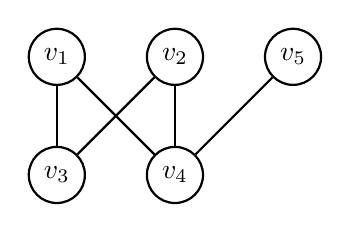
\begin{tikzpicture}[node distance={15mm}, thick, main/.style = {draw, circle}]
        \node[main] (1) {$v_1$};
        \node[main] (2) [right of=1] {$v_2$};
        \node[main] (3) [below of=1] {$v_3$};
        \node[main] (4) [below of=2] {$v_4$};
        \node[main] (5) [right of=2] {$v_5$};
        
        \draw (1) -- (3);
        \draw (1) -- (4);
        \draw (2) -- (3);
        \draw (2) -- (4);
        \draw (4) -- (5);
    \end{tikzpicture}
    \caption{Bipartite graph}
    \label{f_graphs_bipartite}
\end{subfigure}
\begin{subfigure}[b]{0.45\textwidth}
    \centering
    % TikZ code for the second graph
    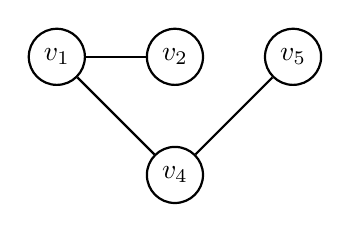
\begin{tikzpicture}[node distance={15mm}, thick, main/.style = {draw, circle}]
        \node[main] (1) {$v_1$};
        \node[main] (2) [right of=1] {$v_2$};
        \node[main] (4) [below of=2] {$v_4$};
        \node[main] (5) [right of=2] {$v_5$};
        \draw (1) -- (2);
        \draw (4) -- (1);
        \draw (5) -- (4);
    \end{tikzpicture}
    \caption{Subgraph of graph (a)}
    \label{f_graphs_subgraph}
\end{subfigure}    
    % Add more subfigures as needed
    \caption{Examples of different graphs. Graphs (a) to (e) exhibit different characteristics, and graph (f) is a subgraph of the undirected graph (a).}
    \label{f_graphs}
\end{figure}

Figure \ref{f_graphs} shows examples of graphs with different characteristics. Several of these attributes can coexist within the same graph. For example, the graph in Figure \ref{f_graphs_multi} is a directed multigraph.

Another critical aspect of graph theory is the concept of subgraphs. A graph $G' = (V', E')$ is called a subgraph of $G = (V,E)$ if $V' \subseteq V$ and $E' \subseteq E$ \cite{diestel_graph_2017}. For example, Figure \ref{f_graphs_subgraph} portrays a subgraph derived from the graph in Figure \ref{f_graphs_undirected}. 

%In the application of functions on graphs, an important type of a subgraph is the local neighborhood of a node. - Not really a subgraph though

For a node $v_i \in V$, the local neighborhood $N_1(v_i) = \{v_j \in V | (v_i, v_j) \in E\}$ \cite{wu_comprehensive_2021} consists of those nodes adjacent to $v_i$. The local neighborhood $N_1(v_i)$ is also referred to as the $1$-hop-neighborhood of $v_i$ because it exclusively contains nodes at a distance of $1$ edge from $v_i$ \cite{bronstein_geometric_2021}. More broadly, the $k$-hop-neighborhood $N_k(v_i)$ of a node $v_i$ encompasses nodes connected to $v_i$ by walks with a length of at most $k$. 

% Wrap up by transitioning to static graphs

As previously discussed, graphs provide a foundational framework for representing relationships between objects. Describing these connections as sets of nodes and edges allows modeling data from many different domains and with various shapes and forms \cite{bronstein_geometric_2017, kazemi_representation_2019}. Such graphs are commonly known as \textit{static graphs} \cite{kazemi_representation_2019, rossi_temporal_2020, you_roland_2022} because they capture relationships that remain constant. 

However, the world around us rarely remains static; it continuously evolves, adapts, and undergoes change. To address the need for modeling these dynamic transformations, the concepts of static graphs are extended by a temporal dimension to encompass \textit{dynamic graphs}. Dynamic graphs introduce the element of time, allowing the capture of how relationships evolve and persist over time, providing a richer, more nuanced understanding of interconnected systems, closely mirroring real-world processes \cite{you_roland_2022, xu_inductive_2020, trivedi_dyrep_2019}.

Two main approaches for modeling dynamic graphs have been proposed: First, modeling evolving graphs as a series of different static snapshots of a graph, so-called \glspl{dtdg}. Second, as a timed list of interaction events, so-called \glspl{ctdg} \cite{rossi_temporal_2020, trivedi_dyrep_2019}. In the following sections, these approaches are explored comprehensively to establish the foundation for the contents of this work.

\subsubsection{Discrete Time Dynamic Graphs}
\label{s_Background_Graphs_DTDGs}
\glspl{dtdg} represent dynamic graphs as a series of static graph snapshots captured at different points in time \cite{rossi_temporal_2020}. These snapshots are usually taken with a constant temporal distance \cite{souza_provably_2022}. While each snapshot represents a static view on the graph at a particular time, the changes between the snapshots represent the dynamic component. Formally, a dynamic graph in discrete-time representation is defined as $\mathcal{G} = \{G_t | t = 1,...,T\}$, where $T$ denotes the number of timestamps for which a snapshot is recorded \cite{you_roland_2022}. Each snapshots represents a static graph $G_t = (V_t, E_t)$ with $V_t = \{v \in V | \tau_v = t\}$ and $E_t = \{e \in E | \tau_e = t\}$ at a specific time $i \in \{1, ..., T\}$, where each vertex $v$ and edge $e$ carries a timestamp $\tau_v$ and $\tau_e$ \cite{you_roland_2022}. Aggregated across all timestamps, $V$ and $E$ represent the sets of nodes and edges, respectively. Furthermore, in an attributed \gls{dtdg} each snapshot is associated with node features $F_t^{vertex} = \{f_{v,t}^{vertex} | v \in V_t\}$ and edge features $F_t^{edge} = \{f_{e,t}^{edge} | e \in E_t\}$. Compared to its static counterpart, the temporal $1$-hop-neighborhood $N_1(v_i, t) = \{v_j \in V_t | (v_i, v_j) \in E_t\}$ of a node $v_i \in V$ also depends on the time $t$. Using the \gls{dtdg} representation, node and edge additions and deletions, as well as attribute updates to node and edge features can be modeled. Figure \ref{f_dtdg}.


\begin{figure}[h]
    \centering
\begin{subfigure}[b]{0.3\textwidth}
    \centering
    % TikZ code for the first graph
    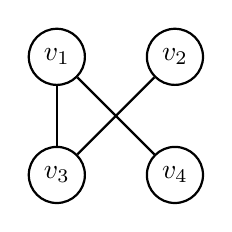
\begin{tikzpicture}[node distance={15mm}, thick, main/.style = {draw, circle}]
        \node[main] (1) {$v_1$};
        \node[main] (2) [right of=1] {$v_2$};
        \node[main] (3) [below of=1] {$v_3$};
        \node[main] (4) [below of=2] {$v_4$};
        \draw (1) -- (3);
        \draw (1) -- (4);
        \draw (2) -- (3);
    \end{tikzpicture}
    \caption{Snapshot $G_1$}
    \label{f_dtdg_1}
\end{subfigure}
\begin{subfigure}[b]{0.3\textwidth}
    \centering
    % TikZ code for the second graph
    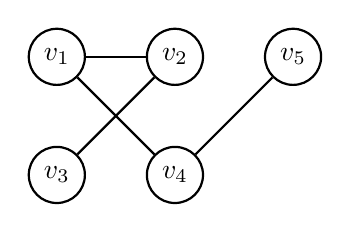
\begin{tikzpicture}[node distance={15mm}, thick, main/.style = {draw, circle}]
        \node[main] (1) {$v_1$};
        \node[main] (2) [right of=1] {$v_2$};
        \node[main] (3) [below of=1] {$v_3$};
        \node[main] (4) [below of=2] {$v_4$};
        \node[main] (5) [right of=2] {$v_5$};
        \draw (1) -- (2);
        \draw (1) -- (4);
        \draw (2) -- (3);
        \draw (4) -- (5);
    \end{tikzpicture}
    \caption{Snapshot $G_2$}
    \label{f_dtdg_2}
\end{subfigure}
\begin{subfigure}[b]{0.3\textwidth}
    \centering
    % TikZ code for the second graph
    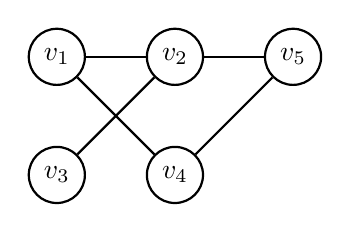
\begin{tikzpicture}[node distance={15mm}, thick, main/.style = {draw, circle}]
        \node[main] (1) {$v_1$};
        \node[main] (2) [right of=1] {$v_2$};
        \node[main] (3) [below of=1] {$v_3$};
        \node[main] (4) [below of=2] {$v_4$};
        \node[main] (5) [right of=2] {$v_5$};
        \draw (1) -- (2);
        \draw (1) -- (4);
        \draw (2) -- (3);
        \draw (2) -- (5);
        \draw (4) -- (5);
    \end{tikzpicture}
    \caption{Snapshot $G_3$}
    \label{f_dtdg_3}
\end{subfigure}
    % Add more subfigures as needed
    \caption{Example of a \gls{dtdg} $\mathcal{G}=\{G_1, G_2, G_3\}$ at different snapshots. Between $G_1$ and $G_2$ the edge $\{v_1, v_3\}$ is removed, node $v_5$ is added and edges $\{v_1, v_2\}$ and $\{v_4, v_5\}$ are added. From $G_2$ to $G_3$ another edge $\{v_2, v_5\}$ is added.}
    \label{f_dtdg}
\end{figure}

While \glspl{dtdg} offer simplicity and ease of processing through their snapshot-based representation \cite{kazemi_representation_2019}, they inherently sacrifice detailed structural information, leading to a coarser depiction of temporal data \cite{trivedi_dyrep_2019, kazemi_representation_2019}. Consequently, they may struggle to capture small and irregular temporal changes \cite{trivedi_dyrep_2019, souza_provably_2022}. Moreover, selecting an appropriate granularity for taking snapshots often results in suboptimal representations \cite{trivedi_dyrep_2019}. Reducing the time interval between snapshots can mitigate these limitations. Still, it introduces complexity by including the entire static graph in each snapshot, leading to parameter redundancy due to shared nodes and edges between snapshots.

\subsubsection{Continuous Time Dynamic Graphs}
\label{s_Background_Graphs_CTDGs}

\glspl{ctdg} offer a high temporal granularity \cite{trivedi_dyrep_2019} and are efficiently represented as sequence of timestamped events $\mathcal{G} = \{\varepsilon_{1}, \varepsilon_{2}, ...\}$ \cite{rossi_temporal_2020}. Following Rossi et al. \cite{rossi_temporal_2020}, each event $\varepsilon_{i}$ is associated with a timestamp $t_i$ with $t_1 \leq t_2 \leq ...$, and it represents either a node-wise occurrence or an interaction. An interaction event $\varepsilon_{i} = \{e_j, f^{edge}_{e_j, t_i}, type_{i}, t_i\}$ signifies the addition, deletion, or feature update of an edge $e_j$, with a defined event type $type_{i} \in \{\mathrm{add}, \mathrm{delete}, \mathrm{update}\}$ and associated edge features $f^{edge}_{e_j, t_i}$ of edge $e_j$ at timestamp $t_i$. A node-wise event $\varepsilon_{i} = \{v_j, f^{vertex}_{v_j, t_i}, type_{i}, t_i\}$ expresses a node addition, deletion, or feature update, where $f^{vertex}_{v_j, t_i}$ represents the features of node $v_j$ at $t_i$. The node set $V$ and the edge set $E$ contain all nodes and edges respectively, that are part of any event in $\mathcal{G}$. For any timestamp $t_i$ a snapshot $G_{t_i}$ of $\mathcal{G}$ at that particular time is defined by all past events $\mathcal{G}(t_i) = \{\varepsilon_{j} | j = 1,...,i\}$.

Similar as in \glspl{dtdg}, the temporal $1$-hop-neighborhood of a node $v_i \in V$ is defined as $N_1(v_i, t) = \{v_j \in V_t | (v_i, v_j) \in E_t\}$, where $V_t$ is the node set and $E_t$ the edge set in the snapshot $G_t$. Analogous to the static representation, the temporal-$k$-hop-neighborhood consists of those nodes $v_j \in V_t$ that are connected to $v_i$ with a walk in $E_t$ that has a length of at most $k$. Extending this concept to the events in a \gls{ctdg}, the temporal $k$-hop-neighborhood $N_k(\varepsilon_i)$ of an event $\varepsilon_{i}$ consists of those events $\varepsilon_{j} \in \mathcal{G}(t_i) \setminus \varepsilon_{i}$ where any node in event $\varepsilon_{i}$ is in the temporal $k$-hop-neighborhood of any node in the event $\varepsilon_{j}$.

\begin{table}[h]
    \centering
    \begin{tabular}{|l|l|}
        \hline
        Event & Description \\
        \hline
        $\varepsilon_{1} = \{v_1, f^{vertex}_{v_1, t_1}, \mathrm{add}, t_1\}$ & Add vertex $v_1$\\
        $\varepsilon_{2} = \{v_2, f^{vertex}_{v_2, t_2}, \mathrm{add}, t_2\}$ & Add vertex $v_2$\\
        $\varepsilon_{3} = \{v_3, f^{vertex}_{v_3, t_3}, \mathrm{add}, t_3\}$ & Add vertex $v_3$\\
        $\varepsilon_{4} = \{e_1 = \{v_1, v_3\}, f^{edge}_{e_1, t_4}, \mathrm{add}, t_4\}$ & Add edge $e_1$ between vertices $v_1$ and $v_3$\\
        $\varepsilon_{5} = \{e_2 = \{v_2, v_3\}, f^{edge}_{e_2, t_5}, \mathrm{add}, t_5\}$ & Add edge $e_2$ between vertices $v_3$ and $v_3$\\
        $\varepsilon_{6} = \{v_4, f^{vertex}_{v_4, t_6}, \mathrm{add}, t_6\}$ & Add vertex $v_4$\\
        $\varepsilon_{7} = \{e_1 = \{v_1, v_3\}, f^{edge}_{e_1, t_7}, \mathrm{delete}, t_7\}$ & Remove edge $e_i$ between vertices $v_1$ and $v_3$\\
        $\varepsilon_{8} = \{v_1, f^{vertex}_{v_1, t_8}, \mathrm{delete}, t_8\}$ & Remove vertex $v_1$\\
        $\vdots$ & $\vdots$ \\
    \end{tabular}
    \caption{Sequence of events comprising an example graph $\mathcal{G}.$}
    \label{t_ctdg_events}
\end{table}

\begin{figure}[ht]
    \centering
\begin{subfigure}[b]{0.3\textwidth}
    \centering
    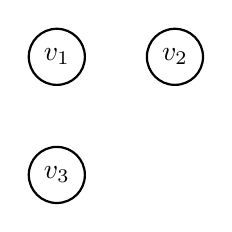
\begin{tikzpicture}[node distance={15mm}, thick, main/.style = {draw, circle}]
        \node[main] (1) {$v_1$};
        \node[main] (2) [right of=1] {$v_2$};
        \node[main] (3) [below of=1] {$v_3$};
    \end{tikzpicture}
    \caption{$G_{t_3}$}
    \label{f_ctdg_1}
\end{subfigure}
\begin{subfigure}[b]{0.3\textwidth}
    \centering
    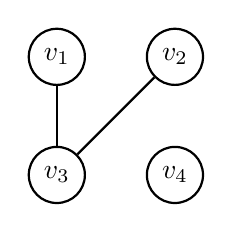
\begin{tikzpicture}[node distance={15mm}, thick, main/.style = {draw, circle}]
        \node[main] (1) {$v_1$};
        \node[main] (2) [right of=1] {$v_2$};
        \node[main] (3) [below of=1] {$v_3$};
        \node[main] (4) [below of=2] {$v_4$};
        \draw (1) -- (3);
        \draw (2) -- (3);
    \end{tikzpicture}
    \caption{$G_{t_6}$}
    \label{f_ctdg_2}
\end{subfigure}
\begin{subfigure}[b]{0.3\textwidth}
    \centering
    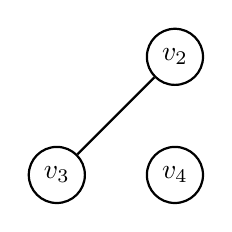
\begin{tikzpicture}[node distance={15mm}, thick, main/.style = {draw, circle}]
        \node[main] (3) {$v_3$};
        \node[main] (4) [right of=3] {$v_4$};
        \node[main] (2) [above of=4] {$v_2$};
        \draw (2) -- (3);
    \end{tikzpicture}
    \caption{$G_{t_8}$}
    \label{f_ctdg_3}
\end{subfigure}
    \caption{Different example snapshots of the graph $\mathcal{G}$ from Table \ref{t_ctdg_events} at timestamps $t_3$, $t_6$ and $t_8$.}
    \label{f_ctdg}
\end{figure}

Table \ref{t_ctdg_events} and Figure \ref{f_ctdg} illustrate an example \gls{ctdg} $\mathcal{G}$. Table \ref{t_ctdg_events} demonstrates that this representation provides a highly detailed yet compact depiction of the dynamic graph evolution. This is a significant advantage over the representation as \gls{dtdg} \cite{trivedi_dyrep_2019}. However, it comes with the drawback that evaluating the graph's state at any given timestamp necessitates the examination of all past events and the assembly of the graph at that specific moment.


\subsection{Geometric Deep Learning}
\label{s_Background_GeometricDeepLearning}


A major hurdle for applying deep learning methods to graphs lies in their underlying non-euclidean structure \cite{wu_comprehensive_2021}. This means that graph data cannot be mapped to an Euclidean space $\mathbb{R}^n$ (for some dimension $n$). Geometric deep learning extends deep neural networks to non-Euclidean domains, providing a framework for working with graph data \cite{bronstein_geometric_2017, bronstein_geometric_2021}. The core principle in geometric deep learning is to leverage inherent symmetries in data to improve the performance of deep learning approaches \cite{bronstein_geometric_2021}. These inherent symmetries are used as inductive biases for deep models, which means that the models are designed in such a way that they can take advantage of the symmetries \cite{bronstein_geometric_2021}. Symmetries are transformations of the input data that leave the underlying structure and relationships in the data unchanged \cite{bronstein_geometric_2021}. These transformations can include translations, rotations, reflections, and other geometric operations. When the output of a function remains unchanged for symmetric data instances, it is referred to as invariant to that transformation. For instance, an image classification model that is invariant to rotations recognizes an object in an image regardless of its orientation. 

% A symmetry refers to the invariance of specific properties of a system to transformations \cite{bronstein_geometric_2021}. An invariance is a property of a model that remains unchanged under certain transformations. For instance, an image classification model that is invariant to rotations recognizes an object in an image regardless of its orientation. 


The key structural property of graphs is that nodes in a graph are provided without a fixed order \cite{bronstein_geometric_2021}. This means that the output of functions on graphs should be independent of the order of the nodes \cite{bronstein_geometric_2021}. A function that satisfies this condition is called a permutation invariant function \cite{bronstein_geometric_2021}. An example of a permutation invariant function on a set of numbers is the arithmetic mean function, which provides the same output regardless of the order of the numbers in the set.

Deep learning methods that apply permutation invariant functions to graph data are referred to as \acrfullpl{gnn}. To investigate particular nodes in a graph, for example, to classify them, \glspl{gnn} apply permutation invariant functions over neighborhoods of these nodes \cite{bronstein_geometric_2021}. The following section covers the specifics of how these models translate the findings of geometric deep learning to actual deep neural models.





%The nature of traditional deep learning methods often presents challenges when applied to graph data due to its non-Euclidean characteristics \cite{wu_comprehensive_2021}. That is because even though universal approximation theorems show that sufficiently complex neural networks can approximate diverse high dimensional functions \cite{hornik_multilayer_1989, kratsios_non-euclidean_2020}, finding a good fit in a general neural network is not trivial and gets increasingly difficult with growing neural network sizes \cite{bronstein_geometric_2021}. This problem is referred to as the curse of dimensionality \cite{bellman_dynamic_1966}. Many deep learning techniques have been able to overcome the curse of dimensionality and excelled because they use inductive biases to help the model process data with a specific structure, mostly with Euclidean or grid-like structural organization \cite{bronstein_geometric_2017}. \textit{Geometric deep learning} extends deep neural models to non-Euclidean domains, including unstructured sets, manifolds, and graphs, leveraging their underlying geometry for inductive biases \cite{bronstein_geometric_2017, bronstein_geometric_2021}.
%%To address the need for generalizing deep neural models to non-Euclidean domains, the field of \textit{geometric deep learning} emerges, extending the power of deep learning to domains such as unstructured sets, manifolds, and graphs using their underlying geometry for inductive biases \cite{bronstein_geometric_2017, bronstein_geometric_2021}.

%Geometric deep learning leverages the geometric principles of symmetry, deformation stability, and scale separation to aid deep learning models in learning complex functions \cite{bronstein_geometric_2021}. Symmetry refers to the invariance of specific properties of (physical) systems to transformations \cite{bronstein_geometric_2021}. For instance, in computer vision, object categorization remains unaffected by shifts to images, making shifts a form of symmetry \cite{bronstein_geometric_2021}. Using symmetries as is cannot properly aid deep learning models since exact symmetries are rare in real world data, which usually exhibits a significant degree of noise \cite{bronstein_geometric_2021}. Thus, the principle of deformation stability relaxes the definition of invariance and introduces the notion of similarity between data points \cite{bronstein_geometric_2021}. Deformation stability suggests that to maintain a similar representation for data instances that differ through slight distortions, feature mappings must demonstrate a type of stability \cite{bronstein_geometric_2021}. Lastly, encoding data in a multi-scale, hierarchical manner enables the detection of complex correlations \cite{bronstein_geometric_2021}. Multi-scale decomposition splits the learned function into elementary functions that capture the different facets and hierarchical nature of much data \cite{bronstein_geometric_2021}. Combining these principles provides the basis for learning stable representations of high-dimensional data.

%The critical structural property for applying geometric deep learning to graphs is that the nodes in a graph are assumed to be provided without a fixed order, meaning that the output of functions on graphs should not depend on the ordering of nodes \cite{bronstein_geometric_2021}. This is called \textit{permutation invariance} \cite{bronstein_geometric_2021}. For example, the sum function is a permutation-invariant function that aggregates values over all nodes \cite{bronstein_geometric_2021}, providing a graph-wise output. However, the focus of many tasks on graphs, like node classification of link prediction, is node-wise information, requiring functions that act locally \cite{bronstein_geometric_2021}. Such functions are realized by applying permutation invariant functions over local neighborhoods of the investigated nodes \cite{bronstein_geometric_2021}. 

%Approaches that apply these results to deep learning on graphs are referred to as \glspl{gnn}. The following section covers how these models translate the findings of geometric deep learning to actual deep neural models.

%%The nature of traditional deep learning methods often presents challenges when applied to graph data due to its non-Euclidean characteristics \cite{wu_comprehensive_2021}. Unlike data with inherent Euclidean attributes, such as a vector space structure, an underlying coordinate system, or shift invariance, graph data lacks these essential properties \cite{bronstein_geometric_2017}. Many deep learning techniques have excelled on data that possesses an inherent Euclidean or grid-like structural organization \cite{bronstein_geometric_2017}. To address the need for generalizing deep neural models to non-Euclidean domains, the field of \textit{geometric deep learning} emerges, extending the power of deep learning to domains such as unstructured sets, manifolds, and graphs \cite{bronstein_geometric_2017, bronstein_geometric_2021}.

%% What should I put here exactly? I want to bridge the gap to graph neural networks so it should introduce only the necessary background for that, thus maybe first state the general principle and then what that means for gnns? General principle: "exposing the regularities in data through unified geometric principles that can be applied throughout a wide spectrum of applications"

\subsection{Graph Neural Networks}
\label{s_Background_GNNs}


% Transition from GDL to GNNs. Make a short introduction and later cover how the GDL principles show in the different architectures.

\glspl{gnn} are potent tools for various learning tasks on relational and interaction data. They find successful applications in many domains, including drug discovery \cite{dauparas_robust_2022}, weather forecasting \cite{lam_graphcast_2022}, and reasoning on knowledge graphs \cite{huang_few-shot_2022}. 
%They achieve this performance by exploiting the properties of the permutation group underlying graph data \cite{bronstein_geometric_2021}.

The applications of \glspl{gnn} are diverse, but their tasks are often similar. These common tasks are node, edge, and graph classification, node regression, and link prediction \cite{wu_comprehensive_2021, zhou_graph_2020}.
\begin{itemize}
    \item \textbf{Node, Edge, and Graph classification} are the tasks of learning a function that maps each node, edge, or graph to their corresponding label \cite{kipf_semi-supervised_2017}.
    \item \textbf{Node regression} involves predicting a continuous numerical value associated with a node \cite{thomas_graph_2023}.
    \item \textbf{Link prediction} is the task of predicting the presence or absence of edges between pairs of nodes \cite{liben-nowell_link-prediction_2007}.
\end{itemize}

To accomplish these tasks, \glspl{gnn} typically learn representations for elements of graphs, like nodes and edges \cite{zhou_graph_2020}. Learning these representations allows the models to understand and use the structural information present in graph-structured data. The following sections lay out a generalized view of \glspl{gnn} and present \glspl{gnn} as an encoder-decoder pair.

\subsubsection{Encoder-Decoder Framework}
\label{s_Background_GNNs_EncoderDecoderFramework}

Different existing approaches to \glspl{gnn} use diverse notations and conceptualizations to describe their methodologies. This thesis follows \cite{hamilton_representation_2017} and \cite{kazemi_representation_2019} in describing \glspl{gnn} as an encoder-decoder pair.
%Addressing the diversity in notation and methodology followed by different existing approaches to \glspl{gnn}, this thesis follows \cite{hamilton_representation_2017} and \cite{kazemi_representation_2019} in describing \glspl{gnn} as an encoder-decoder pair. 
In the encoder-decoder framework, the so-called encoder component produces representations for graph elements, referred to as embeddings. The decoder is then tasked with making predictions based on these embeddings. Depending on the graph and task, nodes, edges, relation types, subgraphs, and/or entire graphs are embedded \cite{barros_survey_2023}. In many cases, embeddings are only calculated for nodes. Thus, in the following, only node embeddings are discussed.

Within the encoder-decoder framework, node embeddings are formally defined as: 

\begin{definition}
    \label{d_Embedding}
    An \textbf{Embedding} is a numerical representation $h_v$ for a node $v \in V$ in a graph. This representation commonly consists of one or more numerical scalars, vectors, or matrices \cite{kazemi_representation_2019}. For a given graph $G = (V, E)$, node embeddings are the result of the embedding function $emb: (v, G) \mapsto h_v \hspace{5pt} \forall v \in V$.
\end{definition}

Embeddings should capture and represent the structural and semantic information of nodes, facilitating information propagation, integrating local and global features, and enabling effective graph reasoning in downstream tasks\cite{goyal_graph_2018}. The embedding function $emb$ should thus provide similar embeddings for nodes that have structurally and semantically similar neighborhoods and similar features \cite{goyal_graph_2018, bronstein_geometric_2021}.
%The embedding function $emb$ should thus preserve a sense of proximity defined on the graph \cite{goyal_graph_2018}. 
Often, embeddings take the form of a single vector $h_v \in \mathbf{R}^d$ that has a significantly lower dimensionality than the number of nodes in the graph $d<<|V|$ \cite{goyal_graph_2018}.

The encoder and decoder are defined formally as follows:

\begin{definition}
    \label{d_Encoder}
    Given an input graph $G$, the \textbf{Encoder} is the embedding function that maps each node $v \in V$ to an embedding $h_v$.
    \begin{equation}
        h_v = emb(v, G)
    \end{equation}
\end{definition}

%Oftentimes, the encoder produces embeddings in the form of a single vector $Emb_v = (z_v), z_v \in \mathbf{R}^{n}$ \cite{kazemi_representation_2019}. 
The encoder function typically builds on top of geometric deep learning principles and includes trainable parameters, such as neural network layers or modules. There are many different architectural variants for encoders, which are discussed in more detail in \ref{s_Background_GNNs_GNNArchtectures}. 

\begin{definition}
    \label{d_Decoder}
    Given the embedding function defined by the encoder $emb$, the decoder makes predictions $y$ for a particular task.
    \begin{equation}
        y = Decoder(emb, G)
    \end{equation}
\end{definition}

Like the encoders, decoders often incorporate trainable parameters. The decoder architecture depends on the desired output format and the task it handles. In link prediction, for example, the decoder may predict the likelihood of the existence of an edge, given the embeddings of the nodes in the predicted edge.

\subsubsection{Graph Neural Network Architectures}
\label{s_Background_GNNs_GNNArchtectures}

Fundamental differences in \glspl{gnn} architectures arise in the encoder. While the exact realization of the encoder can be diverse, most approaches build upon the same foundational structure. \glspl{gnn} are structured in so-called \gls{gnn} layers \cite{bronstein_geometric_2021, wu_comprehensive_2021, zhou_graph_2020}. A \gls{gnn} layer is a computational step that aggregates information from neighboring nodes and updates the representation of each node. \gls{gnn} layers operate on the adjacency matrix $A$, and the node features $F^{vertex}$ of a graph $G$ \cite{bronstein_geometric_2021}. Each layer applies a permutation equivariant function $F(F^{vertex}, A)$ by subjecting local neighborhoods $N_1(v_i)$ for each node $v_i \in V$ to a shared permutation invariant function $\sigma$ \cite{bronstein_geometric_2021}. This results in updated features $h_{v_i}^l$ as output of the $l$-th layer of a \gls{gnn}. Consecutive \gls{gnn} layers use the updated node features of previous layers, allowing the aggregation of information from outside the immediate neighborhood of the nodes. The first layer uses the raw node features $h_{v_i}^0 = f^{vertex}_{v_i}, \forall v_i \in V$ as input \cite{hamilton_representation_2017}. On a generalized level, \glspl{gnn} obtain updated node features as:

\begin{equation}
    h_{v_i}^l = \sigma(h_{v_i}^{l-1}, \underset{v_j \in N_1(v_i)}{\oplus} \psi(h_{v_j}^{l-1}, \cdots))
\end{equation}

Here, permutation invariance is achieved by aggregating the features of the local neighborhood $N_1(v_i)$ of node $v_i \in V$ from the previous layer with a permutation invariant function $\oplus$, for example, the sum, mean, or maximum function \cite{bronstein_geometric_2021}. $\sigma$ and $\psi$ usually are learnable functions \cite{bronstein_geometric_2021}. $\psi$ is applied to each node $v_j$ in the local neighborhood of $v_i$ and takes the updated features $h_{v_j}^{l-1}$ from the previous \gls{gnn} layer as input alongside other implementation specific features.

Following Bronstein et al. \cite{bronstein_geometric_2021}, most \glspl{gnn} can be described as derived from one of three types of \gls{gnn} layers, mainly differentiated by how the permutation invariant function $\sigma$ transforms the neighborhood features through different realizations of $\psi$.

\begin{itemize}
    \item \textbf{Convolutional \glspl{gnn}:} In this architecture, information from the local neighborhood is directly aggregated with fixed weights $c_{v_i, v_j}$ that represent the importance of node $v_j$ to the representation of node $v_i$ \cite{bronstein_geometric_2021, wu_comprehensive_2021}.
    \begin{equation}
        h_{v_i}^l = \sigma(h_{v_i}^{l-1}, \underset{v_j \in N_1(v_i)}{\oplus} c_{v_i, v_j} \varphi(h_{v_j}^{l-1}))
    \end{equation}
    
    \item \textbf{Attention-based \glspl{gnn}:} By assigning different weights to neighboring elements, attention-based operators can alleviate noise and enhance the quality of results \cite{zhou_graph_2020}. Weights result from a learnable self-attention mechanism $a$ \cite{bronstein_geometric_2021}.
    \begin{equation}
        h_{v_i}^l = \sigma(h_{v_i}^{l-1}, \underset{v_j \in N_1(v_i)}{\oplus} a(h_{v_i}^{l-1}, h_{v_j}^{l-1}) \varphi(h_{v_j}^{l-1}))
    \end{equation}

    \item \textbf{Message-passing-based \glspl{gnn}:} This architecture treats graph layers as a message-passing process in which nodes directly pass information to their neighbors \cite{wu_comprehensive_2021}. A learneable message function $\psi$ passes information between neighboring nodes \cite{bronstein_geometric_2021}.
    \begin{equation}
        h_{v_i}^l = \sigma(h_{v_i}^{l-1}, \underset{v_j \in N_1(v_i)}{\oplus} \varphi(h_{v_i}^{l-1}, h_{v_j}^{l-1}))
    \end{equation}
\end{itemize}

$\varphi$ is a learnable function. The node embeddings are typically obtained as the updated node features from the final layer of a \gls{gnn} \cite{hamilton_representation_2017}. These embeddings are then used as input to task-specific decoders, which can contain trainable parameters \cite{hamilton_representation_2017}.

\subsection{Temporal Graph Neural Networks}
\label{s_Background_TGNNs}

Compared with static \glspl{gnn}, a \gls{tgnn} adds representation for the temporal dimension of evolving data. Existing approaches for \glspl{tgnn} are differentiated by those that work on \glspl{dtdg} and those that work on \glspl{ctdg}. Many approaches integrate layers developed for static \glspl{gnn} with \glspl{cnn} or \glspl{rnn} to introduce a temporal dimension \cite{wu_comprehensive_2021}. In general, \gls{tgnn} methods learn time-dependent node-embeddings \cite{longa_graph_2023}. These outputs of the last layer of a \gls{tgnn} are considered as such node-embeddings and are referred to as $h_{v_i}(t_j)$, representing the embedding of node $v_i \in V$ at time $t_j$. The following paragraphs introduce a generalization of common approaches for both types of temporal graph representations.

\subsubsection{Temporal Graph Neural Networks for Discrete Time Dynamic Graphs}
\label{s_tgnns_for_dtdgs}
\glspl{tgnn} for \glspl{dtdg} combine an approach for handling snapshots of the entire graph at each time point with a mechanism for learning temporal dependencies across time steps \cite{longa_graph_2023}. The most common approach is to evolve embeddings produced by a static \gls{gnn} over time \cite{longa_graph_2023}. Hence, the permutation invariant function $\sigma$ from static \glspl{gnn} is employed in this context. This function is adjusted to calculate updated features of node $v_i \in V$ at a given time $t \in \{1,...,T\}$ as follows:

\begin{equation}
    \sigma(h_{v_i}^{l-1}(t), \underset{v_j \in N_1(v_i, t)}{\oplus} \psi(h_{v_j}^{l-1}(t), \cdots))
\end{equation}

As in static \glspl{gnn}, $\psi$ is implementation-specific and may take additional features as input. For each timestep $t$, $\sigma$ functions exactly the same way as its counterpart in static \glspl{gnn}, using the snapshot $G_t$ of the dynamic graph at time $t$ as basis.

$\sigma$ is combined with a temporal update function $\phi$ to obtain the updated node features in this setting \cite{you_roland_2022}:
\begin{equation}
    h_{v_i}^l(t) = \phi(h_{v_i}^{l}(t-1), \sigma(h_{v_i}^{l-1}(t), \underset{v_j \in N_1(v_i, t)}{\oplus} \psi(h_{v_j}^{l-1}(t), \cdots)))
\end{equation}
The temporal update function $\phi$ encodes the temporal dynamics \cite{longa_graph_2023} and might take additional arguments depending on the specific implementation. As for the permutation invariant function $\sigma$, various implementations of $\phi$ exist. These include using self-attention \cite{sankar_dysat_2020}, or \glspl{rnn} like a \gls{gru} \cite{you_roland_2022}.

\subsubsection{Temporal Graph Neural Networks for Continuous Time Dynamic Graphs}
\label{s_tgnns_for_ctdgs}
\gls{tgnn} methods for \glspl{ctdg} effectively handle streams of events by integrating methods that refresh a node's representation whenever an event related to that node takes place \cite{longa_graph_2023}. They represent an extension of the message-passing-based approach to \glspl{ctdg}, as they merge and aggregate node representations within temporal neighborhoods \cite{longa_graph_2023}.

While the exact approaches vary significantly \cite{longa_graph_2023}, a relatively generic framework is \gls{tgn} \cite{rossi_temporal_2020}. Since many popular approaches are specific instances of \gls{tgn} \cite{rossi_temporal_2020} or extend upon it \cite{souza_provably_2022}, the following paragraphs describe \glspl{tgnn} on \glspl{ctdg} from the viewpoint of this framework.

\glspl{tgnn} for \glspl{ctdg} introduce two novel concepts: 
Event-specific messages and node-specific state. 
Each node $v_i \in V$ is associated with a time-dependent state vector $s_{v_i}(t)$ that represents all its past interactions \cite{longa_graph_2023}. Whenever an event $\varepsilon_{k}$ that involves node $v_i \in V$ occurs, a message $m_{v_i}(\varepsilon_{k})$ is generated to update its state $s_{v_i}(t_k)$. For an interaction event $\varepsilon_{k}$ between source node $v_i \in V$ and target node $v_j \in V$, it is possible to compute two messages:
\begin{equation}
    m_{v_i}(\varepsilon_{k}) = msg_s(s_{v_i}(t_k^-), s_{v_j}(t_k^-), \varepsilon_{k}), \hspace{15pt} m_{v_j}(\varepsilon_{k}) = msg_t(s_{v_j}(t_k^-), s_{v_i}(t_k^-), \varepsilon_{k})
\end{equation}
$t_k^-$ refers to the time just before $t_k$, meaning that $s_{v_i}(t_k^-)$ is the state of node $v_i$ just before the event $\varepsilon_{k}$ occurs. This formulation distinguishes between source and target nodes to represent directed graphs; however, for undirected graphs, both message functions are used to calculate two separate messages for each node. In the case that the encountered event $\varepsilon_{k}$ is a node-wise event on node $v_i \in V$, a single message is computed:
\begin{equation}
    m_{v_i}(\varepsilon_{k}) = msg_n(s_{v_i}(t_k^-), \varepsilon_{k})
\end{equation}

The message functions $msg_s, msg_t, msg_n$ can be learnable. The messages they produce are used to update the states of the nodes. A message $m_{v_i}(\varepsilon_{k})$ updates the state $s_{v_i}(t_k)$ of node $v_i$ trough a learnable state function $state$:
\begin{equation}
    s_{v_i}(t_k) = state(m_{v_i}(\varepsilon_{k}), s_{v_i}(t_k^-))
\end{equation}

The $state$ function is a \gls{rnn}, often a \gls{lstm} or \gls{gru}.

The state is used to compute node embeddings in the \gls{tgnn} layers. These layers resemble their counterparts from static \glspl{gnn}. On a generalized level, updated node features at time $t$ are calculated as:
\begin{equation}
    h_{v_i}^l(t) = \sigma(h_{v_i}^{l-1}(t), \underset{v_j \in N_1(v_i, t)}{\oplus} \psi(s_{v_j}(t), \cdots))
\end{equation}

Where $\sigma$ and $\psi$ can be learnable. $\psi$ takes the state of neighboring nodes as input, together with other features, depending on the specific implementation. Like in static \glspl{gnn}, the actual mechanisms of this permutation invariant function vary. Popular approaches include using \glspl{rnn} \cite{ma_streaming_2018} and self-attention \cite{rossi_temporal_2020}.

To improve scalability, modern \glspl{tgnn} for \glspl{ctdg} employ strategies like only updating the state periodically with an aggregated version of the messages \cite{rossi_temporal_2020}. There also exist approaches that do not use a separate state component. Instead, they embed nodes directly by combining node features, graph topology, and time embeddings \cite{longa_graph_2023, xu_inductive_2020}, just as in static \glspl{gnn}.




\iffalse
\gls{tgn} have been proposed by \cite{rossi_temporal_2020} and represent a general framework for learning representations in dynamic graphs. The framework consists of different modules

\begin{itemize}
    \item \textbf{Memory.} The purpose of the memory module is to store long-term dependencies specific to each node within the graph. The memory at time $t$ represents each node $v_i$ it has already seen as a vector $s_i(t)$. When a node is first encountered, it is initialized with the zero vector. The memory of node $v_i$ is always updated when an event involving that node occurs, for example, an interaction with another node or an update to the node features of $v_i$.
    \item \textbf{Message Function.} For each event $e_i$ a memory update message is computed for each node involved in $e_i$. For example, in the case of an edge addition even $e_i$, introducing an edge between $I_i = \{v_j, v_k\}$, a memory update message is computed for both nodes $v_j$ and $v_k$. In the case of an interaction event between two nodes $e_i = ((v_j, v_k), t_i, a_i)$ the update message is calculated as
    \begin{center}
        $m_j(t_i) = msg_{src}(s_j(t_i^-), s_k(t^-), \Delta t, a_i)$, $m_k(t_i) = msg_{tgt}(s_k(t_i^-), s_j(t^-), \Delta t, a_i)$.
    \end{center}
    In the case of a node-wise event $e_i = ((v_j), t_i, a_i)$ it is calculated as
    \begin{center}
        $m_j(t_i) = msg_{node}(s_i(t_i^-), t_i, a_i)$.
    \end{center}
    $s_j(t_i^-)$ denotes the memory of node $v_j$ just before time $t_i$, $\Delta t$ refers to the time difference between the last memory update and $t_i$. The functions $msg_{src}, msg_{tgt}, msg_{node}$ can be learnable like a Multilayer perceptron. However, the original TGN model uses a simple concatenation of the inputs.
    \item \textbf{Message Aggregator.} The message aggregator enables batch processing of events. Since one batch consists of events until some time $t$ can include multiple events that involve any node $v_i$, this produces multiple memory update messages $m_i(t_1),...,m_i(t_b)$ for $t_1,...,t_b \leq t$ for that node. The message aggregator aggregates these messages into a single aggregated update message
    \begin{center}
        $\bar{m}_i(t) = agg(m_i(t_1), ..., m_i(t_b))$.
    \end{center}
    The aggregation function $agg$ can be learnable, for example, realized as \gls{rnn}. However, the original TGN model uses one of two simple strategies: Aggregate as only the most recent message or aggregate as the mean of all update messages.
    \item \textbf{Memory Updater.} The memory updated uses the (aggregated) update message $\bar{m}_i(t)$ to update the memory of a node $v_i$.
    \begin{center}
        $s_i(t) = mem(\bar{m}_i(t), s_i(t^-))$
    \end{center}
    $mem$ is a learnable function realized as \gls{rnn}, for example as \gls{lstm} or \gls{gru}.
    \item \textbf{Embedding.} The embedding module produces temporal embeddings $z_i(t)$ for node $v_i$ at time $t$. Because the memory of node $v_i$ is only updated when it partakes in an event, its memory could have become outdated if there were no events involving $v_i$ for an extended period of time. The embedding module circumvents this problem by not providing the memory of a node as embedding but instead computing it as
    \begin{center}
        $z_i(t) = emb(v_i,t) = \sum_{n_j \in \mathcal{N}^k_i([0,t])} h(s_i(t), s_j(t), a_{ij}, ???)$
    \end{center}
    with $h$ being a learnable function.
\end{itemize}
\fi


%Add something on XAI? Maybe would make sense if the problem formulation is undertaken next and not in the methodology section